\documentclass{beamer}
\usepackage[utf8]{inputenc}
\usepackage{url}
\usepackage{hyperref}
\graphicspath{{./fig/aula7}}

% Configurando layout para mostrar codigos C++
\usepackage{listings}
\lstset{
  language=HTML,
  basicstyle=\ttfamily\small, 
  keywordstyle=\color{blue}, 
  stringstyle=\color{red}, 
  commentstyle=\color{red}, 
  extendedchars=true, 
  showspaces=false, 
  showstringspaces=false, 
  numbers=left,
  numberstyle=\tiny,
  breaklines=true, 
  backgroundcolor=\color{green!10},
  breakautoindent=true, 
  captionpos=b,
  xleftmargin=0pt,
}
date{}

\title{Desenvolvimento Web Básico}
\subtitle{Aula 8}

\usetheme{lucid}

\begin{document}
\frame{
 \titlepage
}

%--------------------------------------------------------------------------
\begin{frame}{Na aula de hoje...} 
\tableofcontents 
\end{frame}
\section{Bootstrap}
\begin{frame}{Bootstrap}
  \begin{itemize}
      \item Bootstrap é um framework front-end que fornece estruturas de CSS para a criação de sites e aplicações responsivas de forma rápida e simples. 
      \item Além disso, pode lidar com sites de desktop e páginas de dispositivos móveis da mesma forma.
      \item Originalmente, o Bootstrap foi desenvolvido para o Twitter por um grupo de desenvolvedores liderados por Mark Otto e Jacob Thornton.
      \item Logo e se tornou uma das estruturas de front-end e projetos de código aberto mais populares do mundo.
  \end{itemize}
\end{frame}

%--------------------------------------------------------------
\begin{frame}{Bootstrap}{Como usar?}
\begin{block}{Como usar Bootstrap no meu projeto?}
Basta inserir o link para o CSS do Bootstrap no \textbf{head} da sua página HTML;\vspace{0.3cm}
\textcolor{blue}{\href{https://cdn.jsdelivr.net/npm/bootstrap@5.0.2/dist/css/bootstrap.min.css}{https://cdn.jsdelivr.net/npm/bootstrap@5.0.2/dist/css/bootstrap.min.css}}
\end{block}
  \begin{center}
       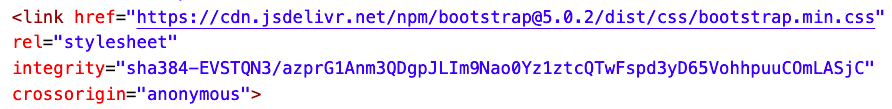
\includegraphics[height=0.14\paperheight]{fig/aula6/aula6_1.png} \\
       \tiny{\textbf{Fonte: } A autora.}
      \end{center}
\end{frame}
%--------------------------------------------
\section{Conteiners}
\begin{frame}{Conteiners Bootstrap}
O Bootstrap 5 requer um elemento container para agrupar o conteúdo do site.\\

\begin{block}{Existem duas classes de contêineres para escolher:}
    \begin{itemize}
        \item A classe \textcolor{blue}{.container} classe fornece um contêiner responsivo de largura fixa;
        \item A classe \textcolor{blue}{.container-fluid} classe fornece um contêiner de largura total, abrangendo toda a largura da viewport.
    \end{itemize}
\end{block}
    \begin{center}
       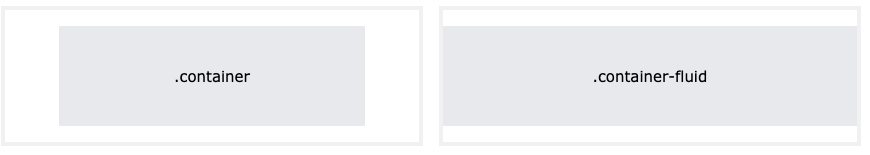
\includegraphics[height=0.2\paperheight]{fig/aula6/aula6_2.png} \\
       \tiny{\textbf{Fonte: } A autora.}
      \end{center}

    
\end{frame}
%--------------------------------------------
\begin{frame}{Conteiners e espaçamento}
Por padrão um Conteiners \underline{não} possuem padding no topo ou dos lados, mas o Bootstrap possui utilidades de espaçamento.

\begin{block}{Classes de espaçamento -\> o que define}
    \begin{itemize}
        \item \textbf{m -\>} a margem
        \item \textbf{p -\>} o padding
        \item \textbf{t -\>} margem superior ou padding superior
        \item \textbf{b -\>} a margem inferior ou padding inferior
        \item \textbf{l -\>} a margem esquerda ou padding esquerdo
        \item \textbf{r -\>} a margem direita ou padding direito
        \item \textbf{x -\>} tanto padding esquerdo como padding direito ou margem esquerda e margem direita
        \item \textbf{y -\>} tanto padding superior e padding inferior ou margem superior e margem inferior.
    \end{itemize}
\end{block}    
\end{frame}
%--------------------------------------------
\begin{frame}{Conteiners e espaçamento}
Exemplo: Adicionando padding ao topo da página\\
\begin{center}
       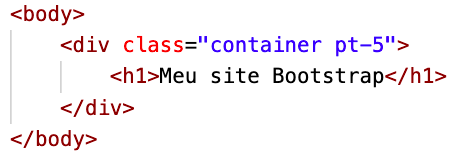
\includegraphics[height=0.37\paperheight]{fig/aula6/aula6_3.png} \\
       \tiny{\textbf{Fonte: } A autora.}
      \end{center}
\end{frame}
%--------------------------------------------
\begin{frame}{Bordas e cores em Conteiners}
É possível criar uma diversidade de containers utilizando classes de borda cor e texto, teste o código:\\
\begin{center}
       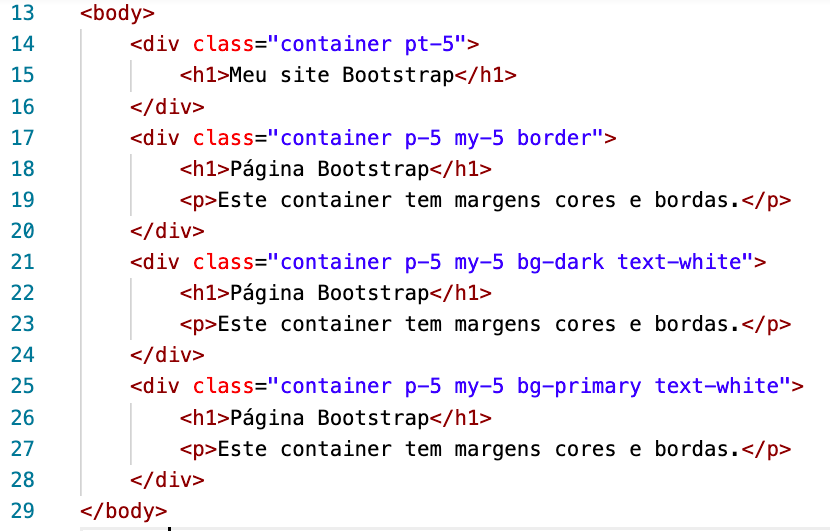
\includegraphics[height=0.4\paperheight]{fig/aula6/aula6_4.png} \\
       \tiny{\textbf{Fonte: } A autora.}
      \end{center}
\end{frame}
%--------------------------------------------
\begin{frame}{Bordas e cores em Conteiners}
Resultado do código:\\
\begin{center}
       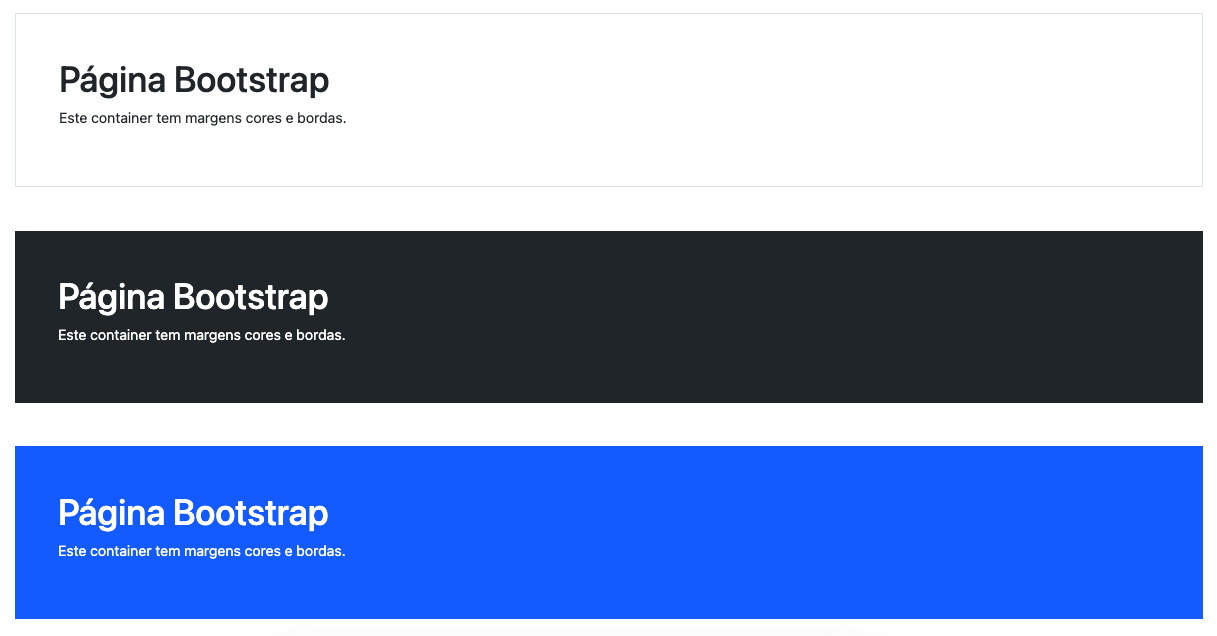
\includegraphics[height=0.5\paperheight]{fig/aula6/aula6_5.png} \\
       \tiny{\textbf{Fonte: } A autora.}
      \end{center}
\end{frame}

%--------------------------------------------
\section{Grid}
\begin{frame}{Sistema de Grid - Bootstrap}
O sistema de grid do Bootstrap é construído com flex-box e permite dividir a sua página em até 12 colunas.\\
\begin{center}
       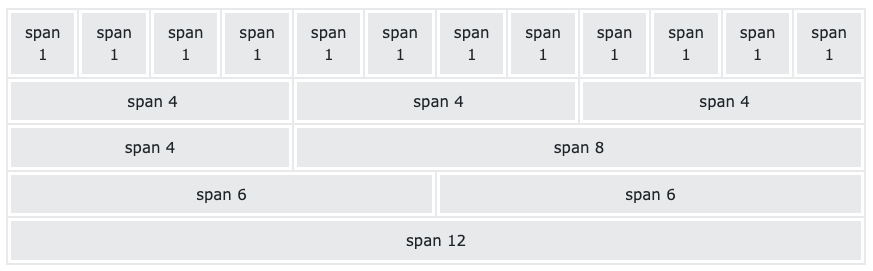
\includegraphics[height=0.35\paperheight]{fig/aula6/aula6_6.png} \\
       \tiny{\textbf{Fonte: } A autora.}
      \end{center}
\end{frame}
%--------------------------------------------

\begin{frame}{Classes de Grid}
Classes CSS para definir grid da página:\\
\begin{itemize}
    \item \textbf{.col-} (dispositivos muito pequenos - largura da tela menor que 576px);
    \item \textbf{.col-sm-} (small devices - largura da tela maior ou igual que 576px);
    \item \textbf{.col-md-} (medium devices - largura da tela maior ou igual que 768px);
    \item \textbf{.col-lg-} (large devices - largura da tela maior ou igual que 992px);
    \item \textbf{.col-xl-} (xlarge devices - largura da tela maior ou igual que 1200px);
    \item \textbf{.col-xxl-} (xxlarge devices - slargura da tela igual ou maior que 1400px);
\end{itemize}
\cite{mdn2023}
\end{frame}
%--------------------------------------------
\begin{frame}{Uso de Classes de Grid}
Exemplo de uso das Classes CSS para definir grid da página:\\
    \begin{center}
       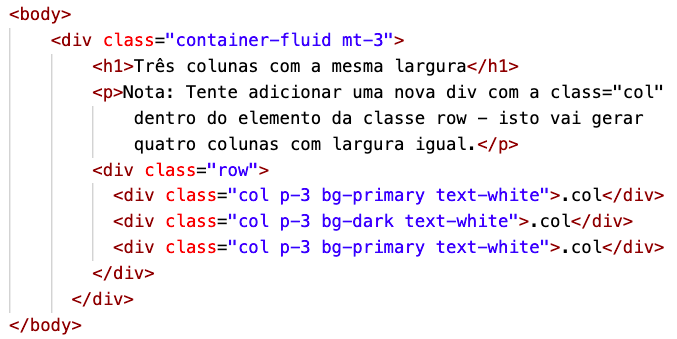
\includegraphics[height=0.5\paperheight]{fig/aula6/aula6_7.png} \\
       \tiny{\textbf{Fonte: } A autora.}
      \end{center}
\end{frame}
%---------------------------------------------------
\section{Topografia}
\begin{frame}{Padrãoes Bootstrap}
Bootstrap 5 usaum valor padrão de font-size de 1rem (16px), e (altura da linha) line-height é 1.5.\\
\vspace{0.5cm}
Todos os elementos <p> possuem margin-top: 0 e margin-bottom: 1rem (16px).\\
Bootstrap tambés estiliza automaticamente elementos h1 até h6.
\cite{wschool2021css}
    
\end{frame}
%---------------------------------------
\begin{frame}{Elementos de cabeçalho}
Também é possível utilizar as classes .display-1 até .display-6 para exibir títulos;
    
\end{frame}

%-----------------------------------------------------------------------
\section{Leitura recomendada}
\begin{frame}{Leitura complementar}
 Para mais informações sobre Git e GitHub, leia:\\
  \vspace{0.6cm}
 \begin{columns}
   \begin{column}{0.4\textwidth}
%      \textbf{Capítulo 29}\\
 \cite{githubpages2022}\\
 E\\
 \cite{beer2015github}.
   \end{column}
   \begin{column}{0.4\textwidth}
   % 
\includegraphics[height=0.7\paperheight]{introgit.jpg} \\
   \end{column}

 \end{columns}
\end{frame}

%----------------------------------------------------------------------------
\section{Referências}

\begin{frame}{Referências}%[allowframebreaks]
\small
\begin{center}
\tiny
\bibliographystyle{apalike}
\bibliography{ref_aula}
\end{center}
\end{frame}

\end{document}

\end{document}